\subsection{Problem Statement}\label{subsec:problem-statement}

NOVA, a relatively new café business, has identified several shortcomings in its current operational infrastructure,
as written in Section~\ref{subsec:the-current-situation}.
Particularly the insights provided by their~\acrfull{epos}.
In an interview with Nancy, the owner of NOVA, transcribed in Appendix~\ref{ch:client-meetings}, it was highlighted
that the business lacks~\acrfull{bi}, a critical tool for decision-making.

The current~\acrshort{epos} does not provide sufficient insights into the data.
Although the data has the specific time stored, as seen in Figure~\ref{fig:nova-csv-data}.
The~\acrshort{epos} does not have the ability to view the data in another scope except daily.

\begin{figure}[H]
    \centering
    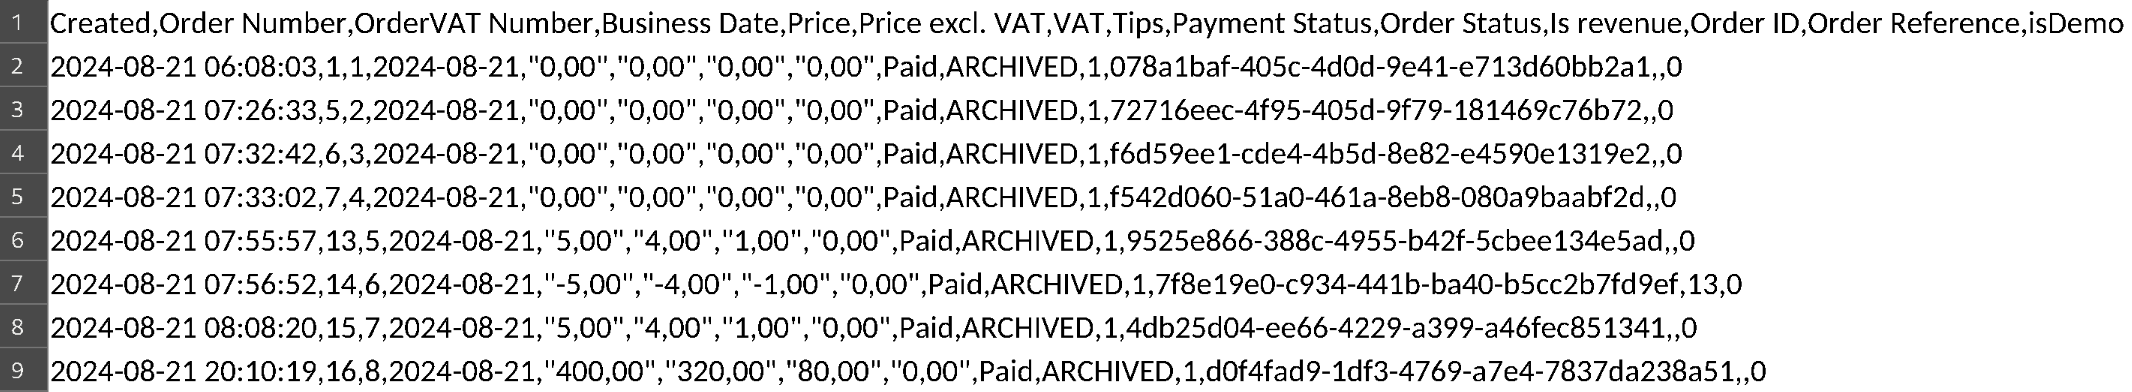
\includegraphics[width=\textwidth]{raw-data}
    \caption{An example of the order csv data that can be exported from NOVA's~\acrshort{epos}.
    }\label{fig:nova-csv-data}
\end{figure}

This lack of insights prevents NOVA from understanding critical operational aspects such as peak business hours and
product-specific demand throughout the day, making it difficult to allocate the staff efficiently and prepare baked
goods.
Without a clear understanding of peak business hours and product-specific demand throughout the day, the café struggles
to allocate staff efficiently and prepare baked goods.
This would lead to either understaffing during peak hours or overstaffing during slower hours, both of which are
having a negative impact on the business.
Additionally, the lack of insights into product-specific demand throughout the day makes it difficult for NOVA to
prepare the right amount of baked goods, resulting in either waste or missed sales opportunities.

Another significant issue is the lack of insights into the effectiveness of the loyalty program.
Without detailed customer data and insights, NOVA cannot evaluate how well the loyalty program is performing.
This hinders their ability to fine-tune the program to improve customer engagement and retention, which is crucial for
the long-term success of the business.

NOVA is in need of a more advanced system that can deliver detailed insights into their sales data, customer behavior,
and loyalty program effectiveness.
The system should provide hourly sales data, product-specific tracking, and tools to evaluate customer behavior,
including the effectiveness of the loyalty program.
Moreover, the system should be user-friendly for all personnel, regardless of their technical proficiency.

This combination of issues highlights the need for a comprehensive and intuitive system that can provide NOVA with the
insights they need to make more informed decisions and improve their operational efficiency.

This presents us with the following problem statement:

\begin{tcolorbox}[title=Problem statement]
    How can we design an application that provides the café owners with a comprehensive overview of their sales and
    facilitates better decision-making based on the available data, while ensuring that the system is intuitive and
    accessible for all users?
\end{tcolorbox}
